\documentclass[]{report}   % list options between brackets        
\usepackage{graphicx, listings, color}      % list packages between braces
\graphicspath{ {Images/} }

% type user-defined commands here

\definecolor{codegreen}{rgb}{0,0.6,0}
\definecolor{codegray}{rgb}{0.5,0.5,0.5}
\definecolor{codepurple}{rgb}{0.58,0,0.82}
\definecolor{backcolour}{rgb}{0.95,0.95,0.92}
 
\lstdefinestyle{mystyle}{
    backgroundcolor=\color{backcolour},   
    commentstyle=\color{codegreen},
    keywordstyle=\color{magenta},
    numberstyle=\tiny\color{codegray},
    stringstyle=\color{codepurple},
    basicstyle=\footnotesize,
    breakatwhitespace=false,         
    breaklines=true,                 
    captionpos=b,                    
    keepspaces=true,                 
    numbers=left,                    
    numbersep=5pt,                  
    showspaces=false,                
    showstringspaces=false,
    showtabs=false,                  
    tabsize=2
}
 
\lstset{style=mystyle}

\begin{document}

\title{CAB420 Assignment 1}   % type title between braces
\author{Jarrod Williams (n9722068) and Madeline Miller (n9342401)}         % type author(s) between braces
\maketitle

\chapter{Theory}

Given the following equation,

$$L(w)=-\sum_{i=1}^{N}log(\frac{1}{1+e^{y_i(w^Tx_i+b)}})+\lambda||w||_2^2$$

\section{Finding the Partial Derivative}
Finding the partial derivative $$\frac{\partial L}{\partial w_j}$$

$$\frac{\partial L}{\partial w_j}(-\sum_{i=1}^{N}log(\frac{1}{1+e^{y_i(w^Tx_i+b)}})+\lambda||w||_2^2)$$

As the regulator at the end of the function is a squared L2 norm, it can be derived trivially.

$$\frac{\partial L}{\partial w_j}(-\sum_{i=1}^{N}log(\frac{1}{1+e^{y_i(w^Tx_i+b)}}))+2\lambda w_j$$

Simplify,

$$\frac{\partial L}{\partial w_j}(\sum_{i=1}^{N}log(1+e^{y_i(w^Tx_i+b)}))+2\lambda w_j$$

Using the chain rule,

$$\sum_{i=1}^{N}\frac{\frac{\partial L}{\partial w_j}(1+e^{y_i(w^Tx_i+b)})}{1+e^{y_i(w_jx_{i,j}+b)}}+2\lambda w_j$$

$$\sum_{i=1}^{N}\frac{\frac{\partial L}{\partial w_j}(1)+\frac{\partial L}{\partial w_j}(e^{y_i(w^Tx_i+b)})}{1+e^{y_i(w_jx_{i,j}+b)}}+2\lambda w_j$$

$$\sum_{i=1}^{N}\frac{\frac{\partial L}{\partial w_j}(e^{y_i(w^Tx_i+b)})}{1+e^{y_i(w_jx_{i,j}+b)}}+2\lambda w_j$$

Using the chain rule again,

$$\sum_{i=1}^{N}\frac{y_ix_ie^{y_i(w^Tx_i+b)}}{1+e^{y_i(w_jx_{i,j}+b)}}+2\lambda w_j$$

\section{Finding the Second Partial Derivative}
Finding the second partial derivative $$\frac{\partial^2 L}{\partial w_j\partial w_k}$$

$$\frac{\partial^2 L}{\partial w_j\partial w_k}=\frac{\partial}{\partial w_k}(\sum_{i=1}^{N}\frac{y_ix_ie^{y_i(w^Tx_i+b)}}{1+e^{y_i(w_jx_{i,j}+b)}}+2\lambda w_j)$$

$$\frac{\partial}{\partial w_k}(\sum_{i=1}^{N}\frac{y_ix_ie^{y_i(w^Tx_i+b)}}{1+e^{y_i(w_jx_{i,j}+b)}})$$

$$\sum_{i=1}^{N}\frac{y_ix_i(\frac{\partial}{\partial w_k}e^{y_i(w^Tx_i+b)})}{1+e^{y_i(w_jx_{i,j}+b)}}$$

Using the chain rule,

$$\sum_{i=1}^{N}\frac{e^{y_i(w_kx_i+b)}y_i^2x_i(\frac{\partial}{\partial w_k}(w^Tx_i+b))}{1+e^{y_i(w_jx_{i,j}+b)}}$$

$$\sum_{i=1}^{N}\frac{e^{y_i(w^Tx_i+b)}y_i^2x_iw_kx_i+b}{1+e^{y_i(w_jx_{i,j}+b)}}$$

$$\sum_{i=1}^{N}\frac{e^{y_i(w^Tx_i+b)}y_i^2x_i^2w_k+b}{1+e^{y_i(w_jx_{i,j}+b)}}$$

\section{Proving it's a convex function}

A function can be defined as convex if the Hessian matrix is positive semi-definite. This is defined as,

$$a^THa\equiv\sum_{j,k}a_ja_kH_{j,k}\geq0$$

Where,

$$H_{j,k}=\frac{\partial^2L}{\partial w_j\partial w_k}$$

Using proof by contradiction, 




\chapter{Practice}


\section{Features, Classes, and Linear Regression}
%%%%%%%%%%%%%%%%%%%%
(a) Plot the training data in a scatter plot.
\begin{center}
	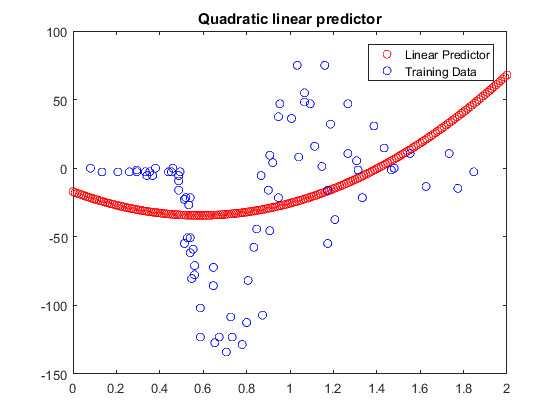
\includegraphics[width=35em]{2_1_Figure_1.png}
	{Figure 2.1.1: Training data in a scatter plot.}
\end{center} 
~\\
(b) Create a linear predictor (assuming quadratic features). Plot it on the same plot as the training data.
\begin{center}
	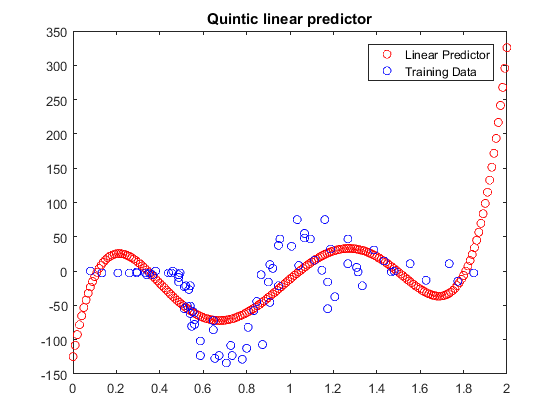
\includegraphics[width=35em]{2_1_Figure_2.png}
	{Figure 2.1.2: Quadratic linear predictor with training data scatter plot.}
\end{center}.
~\\ 
(c) Create another plot with the data and a fifth-degree polynomial.
\begin{center}
	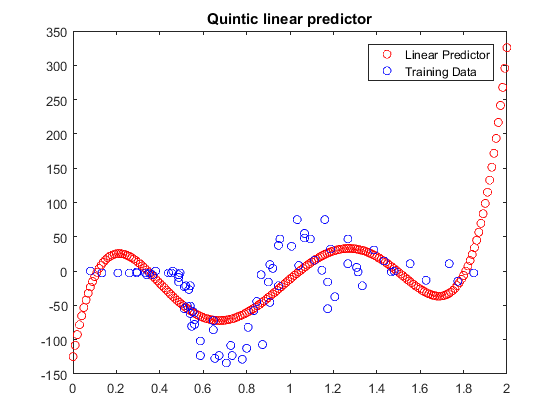
\includegraphics[width=35em]{2_1_Figure_3.png}
	{Figure 2.1.3: Quintic linear predictor with training data scatter plot.}
\end{center}
~\\
(d) Calculate the mean squared error associated with each of your learned models on the training
data.
\begin{lstlisting}[caption=Matlab output for MSE calculations on training data.]
The MSE for the quadratic linear predictor on training data was: 2178.55
The MSE for the quintic linear predictor on training data was: 1254.61
\end{lstlisting}
~\\
(e) Calculate the MSE for each model on the test data (in mcycleTest.txt).
\begin{lstlisting}[caption=Matlab output for MSE calculations on test data.]
The MSE for the quadratic linear predictor on test data was: 1573.27
The MSE for the quintic linear predictor on test data was: 999.65
\end{lstlisting}





\section{kNN Regression}
\section{Hold-out and Cross-validation}
\section{Nearest Neighbor Classifiers}
%%%%%%%%%%%%%%%%%%%%
(a) Plot the data by their feature values, using the class value to select the color.
\begin{center}
	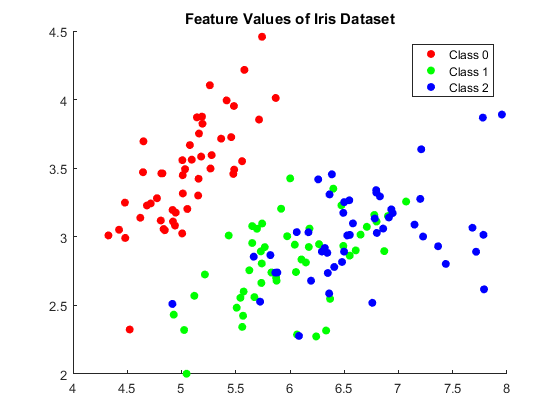
\includegraphics[width=35em]{2_4_Figure_1.png}
	{Figure 2.4.1: Data plotted by feature value with class value determining colour.}
\end{center} 
~\\
(b) Use the provided $knnClassify$ class to learn a 1-nearest-neighbour predictor. Use the function $class2DPlot(learner,X,Y)$ to plot the decision regions and training data together.
\begin{lstlisting}[language=Matlab, caption=Teaching the 1-nearest-neighbour predictor.]
learner = knnClassify(1, X, Y);
class2DPlot(learner,X,Y);
title('1-nearest-neighbour predictor');
\end{lstlisting}
\begin{center}
	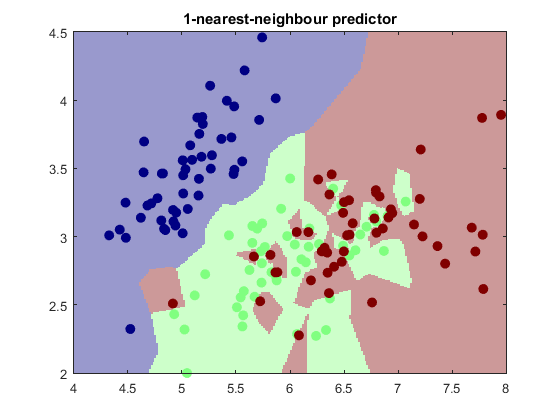
\includegraphics[width=35em]{2_4_Figure_2.png}
	{Figure 2.4.2: Plot of 1-nearest-neighbour predictor. Generated with the code in Listing 2.4.}
\end{center} 
~\\
(c) Do the same thing for several values of k (say, [1, 3, 10, 30]) and comment on their appearance.
\begin{lstlisting}[language=Matlab, caption=Teaching k-nearest-neighbour predictor for multiple values of k. {\bf Note:} figure for 1-nearest-neighbour predictor is above in part (b).]
kValues = [1,3,10,30]; % k=1 is already plotted above in (B).
for index = 1:length(kValues)
    learner = knnClassify(kValues(index), X, Y);
    class2DPlot(learner,X,Y);
    title(strcat(int2str(kValues(index)), '-nearest-neighbour predictor'));
end
\end{lstlisting}
\begin{center}
	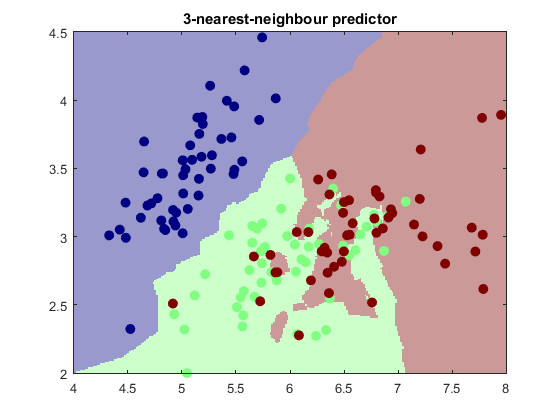
\includegraphics[width=35em]{2_4_Figure_3.png}
	{Figure 2.4.3: Plot of 3-nearest-neighbour predictor. Generated with the code in Listing 2.4.}
\end{center} 
\begin{center}
	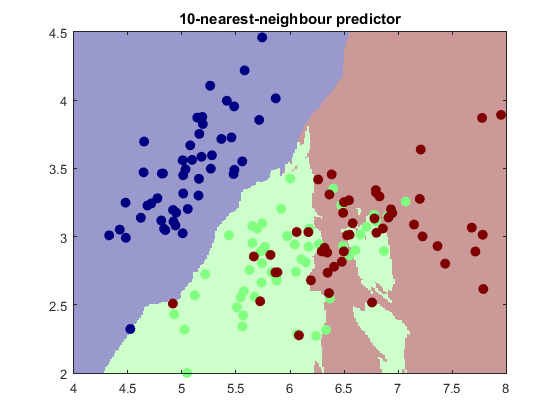
\includegraphics[width=35em]{2_4_Figure_4.png}
	{Figure 2.4.4: Plot of 10-nearest-neighbour predictor. Generated with the code in Listing 2.4.}
\end{center} 
\begin{center}
	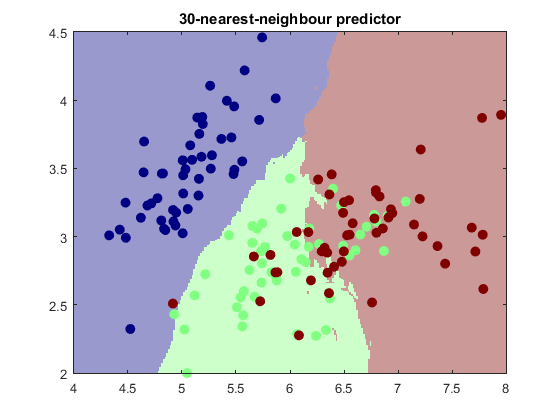
\includegraphics[width=35em]{2_4_Figure_5.png}
	{Figure 2.4.5: Plot of 30-nearest-neighbour predictor. Generated with the code in Listing 2.4.}
\end{center} 
{From visual inspection of figures 2.4.2-2.4.5, as the value of $k$ increases, so does the definition of the decision regions. For small values of $k$ (such as 1), clear under-fitting can be observed. The opposite is also true for large values (such as 30) at which point over-fitting occurs.}
\\~\\
{(d) Now split the data into an 80/20 training/validation split. For k = [1, 2, 5, 10, 50, 100, 200], learn a model on the 80$\%$ and calculate its performance ($\#$ of data classified incorrectly) on the validation data.}
\begin{lstlisting}[language=Matlab, caption=Training models on 80\% training data and calculating its performance on 20\% validation data.]
Xtrain = X(1:118, 1:end);
Xvalid = X(119:end, 1:end);
Ytrain = Y(1:118);
Yvalid = Y(119:end);
kValues = [1, 2, 5, 10, 50, 100, 200];
errors = [];
for index = 1:length(kValues)
    learner = knnClassify(kValues(index), Xtrain, Ytrain); % train model on X/Ytrain
    Yhat = predict(learner, Xvalid); % predict results on Xtrain/Yvalid
    errors = [errors, numel(find(Yhat~=Yvalid))]; % count what fraction of predictions are wrong   
    hold on;
end
\end{lstlisting}
\begin{center}
	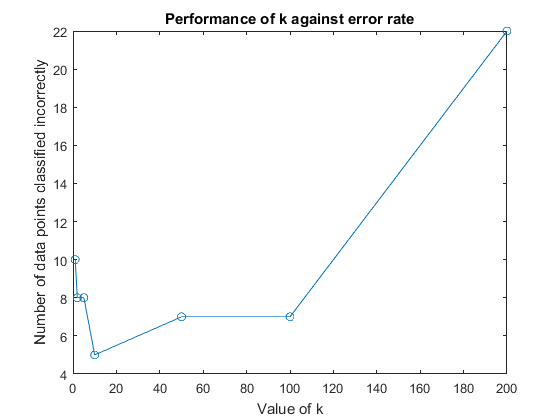
\includegraphics[width=35em]{2_4_Figure_6.png}
	{Figure 2.4.6: Plot of incorrectly classified validation data points against k-nearest-neighbour predictors. Data generated with the code in Listing 2.5.}
\end{center} 
{What value of k appears to generalize best given your training data? Comment on the performance at the two endpoints, in terms of over- or under-fitting.} \\~\\
{For small values of $k$ (1,3,5), under-fitting is present, while larger values (200) provide over-fitting models. As a result, $k$ appears to generalise best between these two values. For Figure 2.4.6 specifically, $k = 10$ appears to generalise best.}




\section{Perceptrons and Logistic Regression}
{(a) Show the two classes in a scatter plot and verify that one is linearly separable while the other is not.}
\begin{center}
	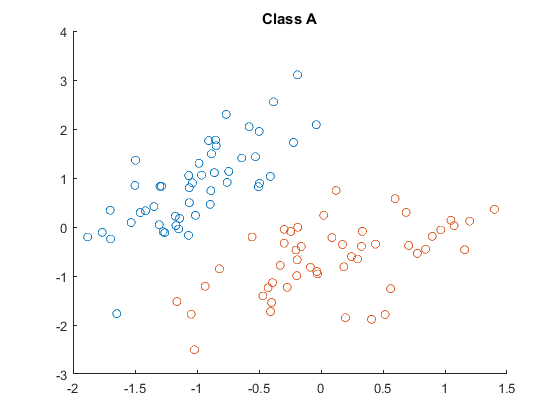
\includegraphics[width=35em]{2_5_Figure_1.png}
	{Figure 2.5.1: Class A. Data {\bf is} linearly separable.}
\end{center} 
\begin{center}
	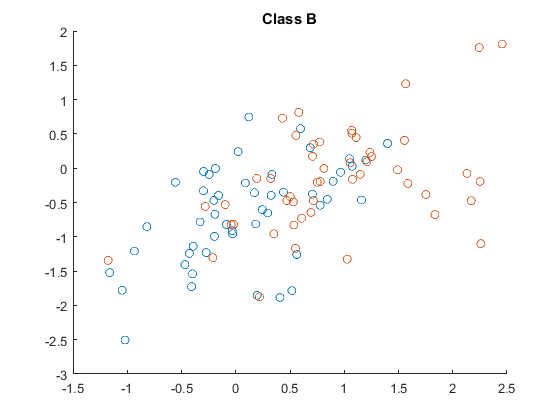
\includegraphics[width=35em]{2_5_Figure_2.png}
	{Figure 2.5.2: Class B. Data {\bf is not} linearly separable.}
\end{center} 
~\\
{(b) Write the function @logisticClassify2/plot2DLinear.m so that it plots the two
classes of data in different colors, along with the decision boundary. Include the listing of your code in your report.}

\begin{lstlisting}[language=Matlab, caption=plot2DLinear() Implementation]
function plot2DLinear(obj, X, Y)
% plot2DLinear(obj, X,Y)
%   plot a linear classifier (data and decision boundary) when features X are 2-dim
%   wts are 1x3,  wts(1)+wts(2)*X(1)+wts(3)*X(2)
%
[n,d] = size(X);
if (d~=2) error('Sorry -- plot2DLogistic only works on 2D data...'); end;

%%% TODO: Fill in the rest of this function...
figure('Name','Linear Plot');
hold on;

% Plot class data.
classes = unique(Y);

classAIndicies = find(Y==classes(1));
xPointsClassA = X(classAIndicies, 1:end);
scatter(xPointsClassA(:, 1), xPointsClassA(:, 2));

classBIndicies = find(Y==classes(2));
xPointsClassB = X(classBIndicies, 1:end);
scatter(xPointsClassB(:, 1), xPointsClassB(:, 2));


% Plot decision boundary.
wts = getWeights(obj);
f = @(x1, x2) wts(1) + wts(2)*x1 + wts(3)*x2 ;
ezplot(f,[-3.5,3.5])

legend('Class 0','Class 1', 'Decision Bondary');
hold off;
\end{lstlisting}
{To demo your function plot the decision boundary corresponding to the classifier: $sign( .5 + 1x_{1} − .25x_{2} )$ along with the A data, and again with the B data.}
\begin{lstlisting}[language=Matlab, caption=Demoing plot2DLinear()]
%% (B) Write the function @logisticClassify2/plot2DLinear.m such that it 
%      can Plot the two classes of data in different colors, along with the 
%      decision boundary (a line). To demo your function plot the decision 
%       boundary corresponding to the classifier sign( .5 + 1x1 − .25x2 )
%       along with the A data, and again with the B data.

learner=logisticClassify2(); % create "blank" learner
learner=setClasses(learner, unique(YA)); % define class labels using YA or YB
wts = [0.5 1 -0.25]; % TODO: fill in values
learner=setWeights(learner, wts); % set the learner's parameters
plot2DLinear(learner, XA, YA);
title('Class A with Decision Boundary');
plot2DLinear(learner, XB, YB);
title('Class B with Decision Boundary');
\end{lstlisting}
\begin{center}
	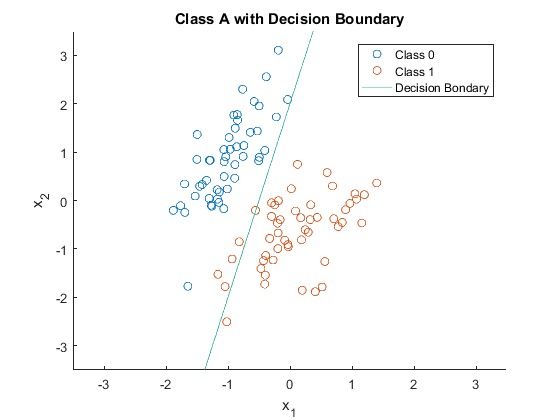
\includegraphics[width=35em]{2_5_Figure_3.png}
	{Figure 2.5.3: Class A with decision boundary plotted.}
\end{center} 
\begin{center}
	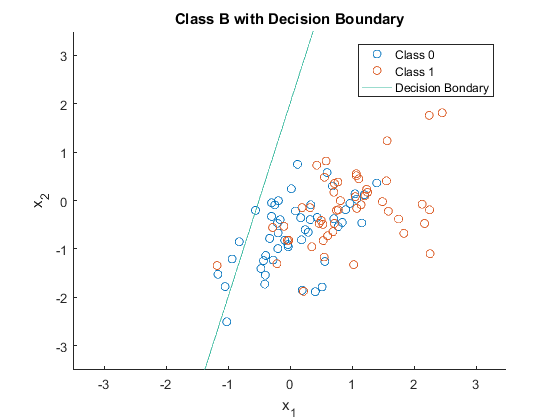
\includegraphics[width=35em]{2_5_Figure_4.png}
	{Figure 2.5.4: Class B with decision boundary plotted.}
\end{center} 
~\\
{(c) Complete the predict.m function to make predictions for your linear classifier.}
\begin{lstlisting}[language=Matlab, caption=predict() Implementation]
function Yte = predict(obj,Xte)
% Yhat = predict(obj, X)  : make predictions on test data X

% (1) make predictions based on the sign of wts(1) + wts(2)*x(:,1) + ...
% (2) convert predictions to saved classes: Yte = obj.classes( [1 or 2] );
wts = getWeights(obj);
yhat = zeros(size(Xte,1),1);
f = @(x1, x2) wts(1) + wts(2)*x1 + wts(3)*x2;

for i=1:size(Xte,1)
    x = sign(f(Xte(i,1),Xte(i,2)));
    yhat(i) = obj.classes(ceil((x+3)/2));
end;

Yte = yhat;
\end{lstlisting}
{Again, verify that your function works by computing \& reporting the error rate of the classifier in the previous part on both data sets A and B. (The error rate on data set A should be ≈ 0.0505.)}
\begin{lstlisting}[language=Matlab, caption=Verifying predict() works]
% Data set A
yte = predict(learner,XA);
classError = 0;
for i=1:size(YA,1);
    if(YA(i) ~= yte(i));
        classError = classError + 1;
    end;
end;
finalClassError = classError/size(YA,1); % = 0.0505
disp(strcat({'The error for class A is:'},{' '},{num2str(finalClassError,' %.4f')}));
% Data set B
yte = predict(learner,XB);
classError = 0;
for i=1:size(YB,1);
    if(YB(i) ~= yte(i));
        classError = classError + 1;
    end;
end;
finalClassError = classError/size(YB,1); % = 0.54555
disp(strcat({'The error for class B is:'},{' '},{num2str(finalClassError,' %.4f')}));
\end{lstlisting}
\begin{lstlisting}[caption=Matlab output for error rate of Class A and B.]
'The error rate for class A is: 0.0505'
'The error rate for class B is: 0.5455'
\end{lstlisting}
~\\
{(d) In my provided code, I first transform the classes in the data Y into "class 0" (negative) and "class 1" (positive). In our notation, let $z = \theta x^{(i)}$ is the linear response of the perceptron, and $\sigma$ is the standard logistic function.
$$\sigma (z) = (1 + exp(-z))^{-1}$$
The (regularized) logistic negative log likelihood loss for a single data point j is then
$$ J_{j}(\theta) = -y^{(j)} log \sigma (\theta x^{(j)T}) - (1 - y^{(j)})log(1-\sigma (\theta x^{(j)T})) + \alpha \sum_{i} \theta^{2}_{i} $$
where $y(j)$ is either 0 or 1. Derive the gradient of the regularized negative log likelihood $J_{j}$
for logistic regression, and give it in your report.
\\~\\
The derivative of the gradient can be found by computing $\frac{\partial J_{j}(\theta)}{\partial \theta_{i}}$ over the surrogate loss for point j, as given by $x^{(j)}$, $y^{(i)}$. The derivative then is as follows:
$$\frac{\partial J_{j}(\theta)}{\partial \theta_{i}} = x^{j}((1+exp(z))^{-1} - y^{(j)}) + 2.\alpha.\theta_{i} $$}
\\~\\
(e) Complete your train.m function to perform stochastic gradient descent on the logistic loss function. This will require that you fill in:
\\~\\
(1) computing the surrogate loss function at each iteration ($J = 1/m\sum J_{j}$)
\begin{lstlisting}[language=Matlab, caption=Calculating surrogate loss at each point.]
iter=1; Jsur=zeros(1,stopIter); J01=zeros(1,stopIter); done=0; 
while (~done) 
  step = stepsize/iter;               % update step-size and evaluate current loss values
  Jsur(iter) = inf;   
  %%% TODO: compute surrogate (neg log likelihood) loss
  wtsTrans = (obj.wts * obj.wts')';
  Jsur(iter) = mean(-Y .* log(logistic(obj, X)) - (1 - Y) .* log(1 - logistic(obj, X)) + reg * sum(wtsTrans));
  J01(iter) = err(obj, X, Yin);
\end{lstlisting}
~\\
(2) computing the prediction and gradient associated with each data point $x^{(i)}, j^{(i)}$;
\begin{lstlisting}[language=Matlab, caption=Compute linear responses and activation for data point j.]
    % Compute linear responses and activation for data point j
    %%% TODO ^^^
    y = logistic(obj,X(j,:));
\end{lstlisting}
~\\
(3) a gradient step on the parameters θ;
\begin{lstlisting}[language=Matlab, caption=Compute gradient.]
    % Compute gradient:
    %%% TODO ^^^
    gradient = X1(j,:) * (y - Y(j)) + 2 * reg * obj.wts;

    obj.wts = obj.wts - step * gradient;      % take a step down the gradient
\end{lstlisting}
~\\
(4) a stopping criterion (usually either stopIter iterations or that J has not changed by more than stopTol since the last iteration through all the data).
\begin{lstlisting}[language=Matlab, caption=Implement stopping criterion.]
  %   done = false;
  %%% TODO: Check for stopping conditions
  deltaJ = mean(-Y .* log(logistic(obj, X)) - (1 - Y) .* log(1 - logistic(obj, X)) + reg * obj.wts * obj.wts');  
  if (iter == stopIter || abs(deltaJ - Jsur(iter)) < stopTol)
    done = true;
  end;
\end{lstlisting}
~\\

(f) Run your logistic regression classifier on both data sets (A and B); for this problem, use no regularization ($\alpha = 0$). Describe your parameter choices (stepsize, etc.) and show a plot of both the convergence of the surrogate loss and error rate, and a plot of the final converged classifier with the data (using e.g. plotClassify2D). In your report, please also include the functions that you wrote (at minimum, train.m, but possibly a few small helper functions as well).

\begin{lstlisting}[language=Matlab, caption=Full train.m implementation.]
function obj = train(obj, X, Y, varargin)
% obj = train(obj, Xtrain, Ytrain [, option,val, ...])  : train logistic classifier
%     Xtrain = [n x d] training data features (constant feature not included)
%     Ytrain = [n x 1] training data classes 
%     'stepsize', val  => step size for gradient descent [default 1]
%     'stopTol',  val  => tolerance for stopping criterion [0.0]
%     'stopIter', val  => maximum number of iterations through data before stopping [1000]
%     'reg', val       => L2 regularization value [0.0]
%     'init', method   => 0: init to all zeros;  1: init to random weights;  
% Output:
%   obj.wts = [1 x d+1] vector of weights; wts(1) + wts(2)*X(:,1) + wts(3)*X(:,2) + ...


  [n,d] = size(X);            % d = dimension of data; n = number of training data

  % default options:
  plotFlag = true; 
  init     = []; 
  stopIter = 100; % Lowered to improve performance. Initially 1000.
  stopTol  = -1;
  reg      = 0.0;
  stepsize = 1;

  i=1;                                       % parse through various options
  while (i<=length(varargin)),
    switch(lower(varargin{i}))
    case 'plot',      plotFlag = varargin{i+1}; i=i+1;   % plots on (true/false)
    case 'init',      init     = varargin{i+1}; i=i+1;   % init method
    case 'stopiter',  stopIter = varargin{i+1}; i=i+1;   % max # of iterations
    case 'stoptol',   stopTol  = varargin{i+1}; i=i+1;   % stopping tolerance on surrogate loss
    case 'reg',       reg      = varargin{i+1}; i=i+1;   % L2 regularization
    case 'stepsize',  stepsize = varargin{i+1}; i=i+1;   % initial stepsize
    end;
    i=i+1;
  end;

  X1    = [ones(n,1), X];     % make a version of training data with the constant feature

  Yin = Y;                              % save original Y in case needed later
  obj.classes = unique(Yin);
  if (length(obj.classes) ~= 2) error('This logistic classifier requires a binary classification problem.'); end;
  Y(Yin==obj.classes(1)) = 0;
  Y(Yin==obj.classes(2)) = 1;           % convert to classic binary labels (0/1)

  if (~isempty(init) || isempty(obj.wts))   % initialize weights and check for correct size
    obj.wts = randn(1,d+1);
  end;
  if (any( size(obj.wts) ~= [1 d+1]) ) error('Weights are not sized correctly for these data'); end;
  wtsold = 0*obj.wts+inf;

% Training loop (SGD):
iter=1; Jsur=zeros(1,stopIter); J01=zeros(1,stopIter); done=0; 
while (~done) 
  step = stepsize/iter;               % update step-size and evaluate current loss values
  Jsur(iter) = inf;   
  %%% TODO: compute surrogate (neg log likelihood) loss
  wtsTrans = (obj.wts * obj.wts')';
  Jsur(iter) = mean(-Y .* log(logistic(obj, X)) - (1 - Y) .* log(1 - logistic(obj, X)) + reg * sum(wtsTrans));
  J01(iter) = err(obj, X, Yin);

  if (plotFlag), switch d,            % Plots to help with visualization
    case 1, fig(2); plot1DLinear(obj,X,Yin);  %  for 1D data we can display the data and the function
    case 2, fig(2); plot2DLinear(obj,X,Yin);  %  for 2D data, just the data and decision boundary
    otherwise, % no plot for higher dimensions... %  higher dimensions visualization is hard
  end; end;
  fig(1); semilogx(1:iter, Jsur(1:iter),'b-',1:iter,J01(1:iter),'g-'); drawnow;

  for j=1:n,
    % Compute linear responses and activation for data point j
    %%% TODO ^^^
    y = logistic(obj,X(j,:));

    % Compute gradient:
    %%% TODO ^^^
    gradient = X1(j,:) * (y - Y(j)) + 2 * reg * obj.wts;

    obj.wts = obj.wts - step * gradient;      % take a step down the gradient
  end;


  %   done = false;
  %%% TODO: Check for stopping conditions
  deltaJ = mean(-Y .* log(logistic(obj, X)) - (1 - Y) .* log(1 - logistic(obj, X)) + reg * obj.wts * obj.wts');  
  if (iter == stopIter || abs(deltaJ - Jsur(iter)) < stopTol)
    done = true;
  end;

  wtsold = obj.wts;
  iter = iter + 1;
end;
\end{lstlisting}
{ As $\alpha$ was set to 0, $stepsize$ was set to 1 and number of iterations was set to 100. Beyond 100 iterations, computation time became too high for minimal improvements to the error  rate and surrogate loss. The logistic regression classifier was then run on both classes:}
\begin{lstlisting}[language=Matlab, caption=Code to run logistic regression classifier on both data sets.]
% Train Class A
train(learner, XA, YA);
legend('Error Rate', 'Surrogate Loss');
% Plot final converged classifier decision boundaries.
figure();
plotClassify2D(learner, XA, YA);

% Train Class B
train(learner, XB, YB);
legend('Error Rate', 'Surrogate Loss');
% Plot final converged classifier decision boundaries.
figure();
plotClassify2D(learner, XB, YB);
\end{lstlisting}



\begin{center}
	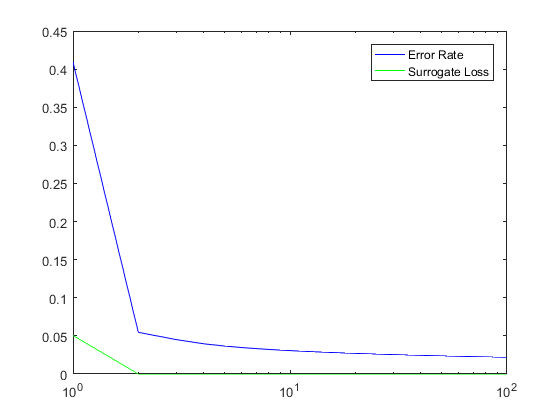
\includegraphics[width=35em]{2_6_Figure_1.png}
	{Figure 2.6.1: Plot of convergence of error rate and surrogate loss for Class A.}
\end{center} 

\begin{center}
	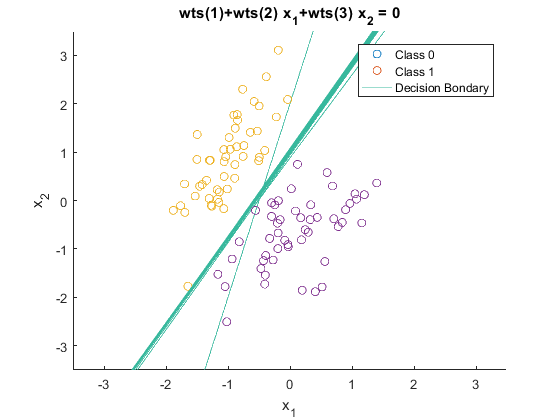
\includegraphics[width=35em]{2_6_Figure_2.png}
	{Figure 2.6.2: Plot of final converged classifier for Class A.}
\end{center} 


\begin{center}
	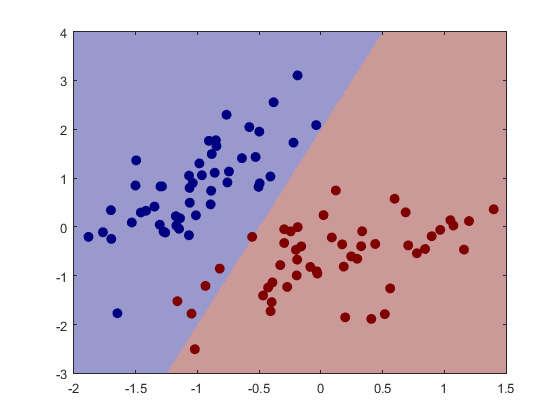
\includegraphics[width=35em]{2_6_Figure_3.png}
	{Figure 2.6.3: Plot of final converged classifier decision boundaries for Class A.}
\end{center} 

\begin{center}
	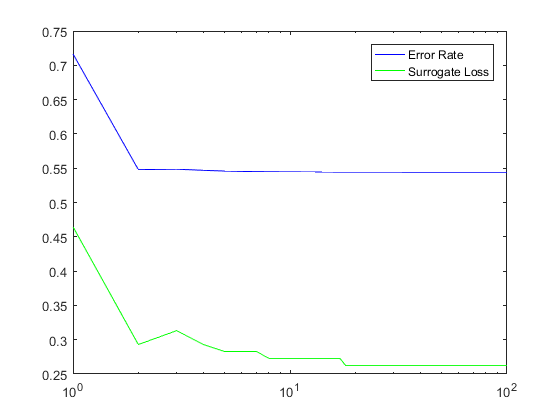
\includegraphics[width=35em]{2_6_Figure_4.png}
	{Figure 2.6.4: Plot of convergence of error rate and surrogate loss for Class B.}
\end{center} 

\begin{center}
	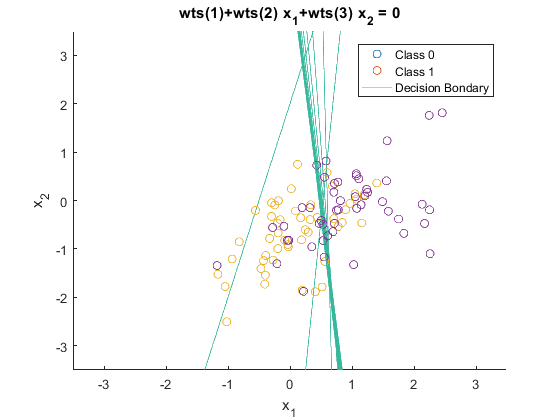
\includegraphics[width=35em]{2_6_Figure_5.png}
	{Figure 2.6.5: Plot of final converged classifier for Class B.}
\end{center} 


\begin{center}
	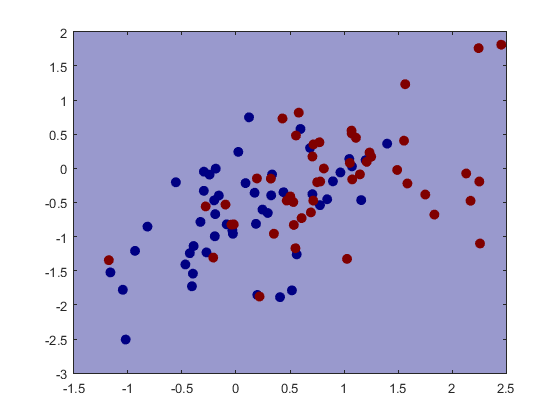
\includegraphics[width=35em]{2_6_Figure_6.png}
	{Figure 2.6.6: Plot of final converged classifier decision boundaries for Class B.}
\end{center} 






\end{document}
